\documentclass[12pt, addpoints]{exam}

\usepackage{hyperref}
\usepackage{mdframed}
\usepackage{graphicx, caption}	
\usepackage{array, multicol, tabu}
\usepackage{amsmath, amsthm}
\usepackage{comment}
\usepackage{enumerate}
\usepackage{url}
\usepackage{textcomp}
\newcommand{\vect}[1]{\mathbf{#1}}
\newcommand{\vstr}{\vspace{\stretch{1}}}
\everymath{\displaystyle}
\setlength{\parindent}{0pt}

\theoremstyle{plain}
\newtheorem{thm}{Theorem}
\newtheorem*{thm*}{Theorem}

\printanswers
\pointformat{\bf(\thepoints)}
\pointpoints{pt}{pts}
\bonuspointformat{\bf(\thepoints)}
\bonuspointpoints{pt}{pts}

\coverfirstpageheader{\bf MATH 2554 (Calculus I) \\
		Spring 2016 \\
		}
		{}
		{{Name:} \underline{\hspace{40ex}} \\
		\vspace{0.5pc}
		Fri 29 Apr 2016}
\coverextraheadheight[2pc]{0in}
\coverfirstpagefooter{}{}{\Large Good luck!}
\coverrunningheader{}
	{Exam 4: Introduction to Integrals}
	{}
\coverrunningheadrule	
\coverrunningfootrule
\coverrunningfooter{Wheeler}{Cal I Spring 2016}{p. \thepage\ (of \numpages)}

\firstpageheader{}
	{Exam 4: Introduction to Integrals}
	{}
\firstpageheadrule
\firstpagefootrule
\firstpagefooter{Wheeler}{Cal I Spring 2016}{p. \thepage\ (of \numpages)}

\runningheadrule
\runningheader{}
	{Exam 4: Introduction to Integrals}
	{}
\runningfootrule
\runningfooter{Wheeler}{Cal I Spring 2016}{p. \thepage\ (of \numpages)}

\title{\vspace{-8pc}
\vfill{\Huge
	\bf Exam 4: Introduction to Integrals (\S 4.7,\ 4.9-5.4)} 
	}
%\author{}
\date{}

% % % % % % % % % % % % % % % % % % % %
\begin{document}

\begin{coverpages}
\maketitle
\thispagestyle{headandfoot}
\vspace{-4pc}
{\bf Exam Instructions:} You have 50 minutes to complete this exam.  Justification is required for all problems.  Notation matters!  You will also be penalized for missing units and rounding errors.  No electronic devices (phones, iDevices, computers, etc) except for a \textbf{basic scientific calculator}.  On story problems, round to one decimal place. %If you finish early then you may leave, UNLESS there are less than 5 minutes of class left.  To prevent disruption, if you finish with less than 5 minutes of class remaining then please stay seated and quiet.

\begin{flushright}
In addition, please provide the following data:

\vspace{0.3in}
Drill Instructor: \underline{\hspace{40ex}}

\vspace{0.3in}
Drill Time: \underline{\hspace{40ex}}
\end{flushright}

\vfill
\textbf{Your signature below indicates that you have read this page and agree to follow the Academic Honesty Policies of the University of Arkansas.}  

\vspace{0.3in}
Signature: {\bf (1 pt)} \underline{\hspace{73ex}}

% % % % % % % % % %
\newpage

\begin{center}
\vspace*{\fill}
%\gradetable
\vspace*{\fill}
\end{center}
\end{coverpages}

% % % % % % % % % % % % % % % % % % % %
\begin{questions}
\thispagestyle{headandfoot}
% % % % %
\question[10] Use geometry to evaluate $\int_{-2}^3|x+1|\ dx$.
\begin{solutionbox}
%\vspace
{3.55in}
\vspace{-1.9pc}
\begin{center}
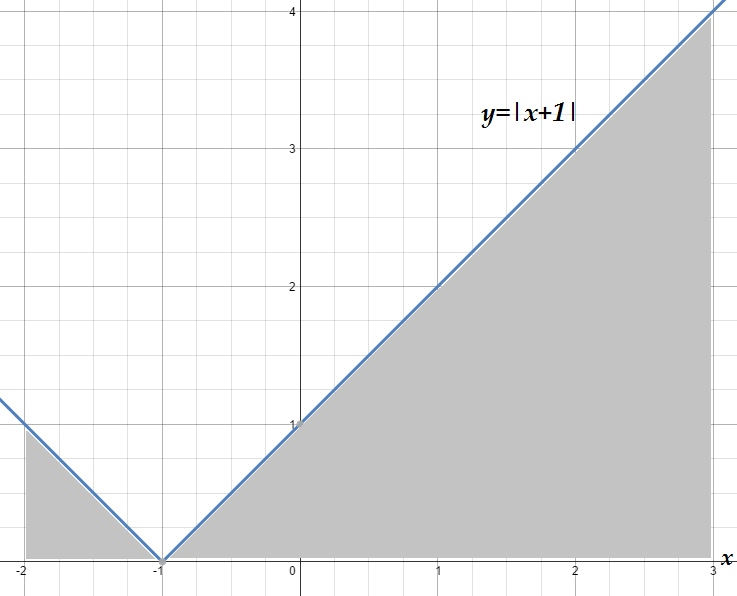
\includegraphics[scale=0.5]{exam4Sec5p2}
\end{center}

\vspace{-1pc}
The indefinite integral is the combined area of the shaded triangles:
\vspace{-0.5pc}
\[
\frac{1}{2}\left(1\times 1\right)+\frac{1}{2}\left(4\times 4\right)=\frac{1}{2}+8=\boxed{\frac{17}{2}}
\]
\end{solutionbox}
\vstr 

% % % % % 
\question \emph{For this problem, you are not required to simplify answers.}  Runners A and B are running a race in which Runner B has a head start.  Their respective velocity functions and initial position functions are
\vspace{-0.5pc}
\begin{align*}
\text{Runner A: }& v(t) =2at\text{ m/s,} \quad s(0) =0 \text{ m,} \\
\text{Runner B: }& V(t) =b\text{ m/s,} \quad S(0) =c \text{ m,}
\end{align*}

\vspace{-1.25pc}
where $a,b,c>0$ are all constants, and $t$ is in seconds.

\begin{parts}
% % %
\part[4] Find the initial velocity of each of the runners.
\begin{solutionbox}
%\vspace
{0.75in}
\vspace{-2pc}
\begin{align*}
\text{Runner A: }& v(0) =2a(0)=\boxed{0 \text{ m/s}} \\
\text{Runner B: }& V(0) =b=\boxed{b \text{ m/s}} 
\end{align*}
\end{solutionbox}
\vstr

% % %
\part[6] Find the position function of each of the runners.
\begin{solutionbox}
%\vspace
{3.1in}
\vspace{-2pc}
\begin{align*}
\text{Runner A: }& s(t) =\int v(t)\ dt =\int 2at\ dt \\
	& =at^2+C \\
S(0) &=a(0)^2+C=0 \\
	&\implies C=0 \\
	&\boxed{s(t) =at^2 \text{ m}} \\	
\text{Runner B: }& S(t) =\int V(t)\ dt =\int b\ dt \\
	& =bt+C \\
S(0) &=b(0)+C=c \\
	&\implies C=c \\
	&\boxed{S(t) =bt+c \text{ m}} \\
\end{align*}
\end{solutionbox}
\vstr 

% % %
\part[3] Does Runner A ever catch up to Runner B?  If so, at what time and what position?
\begin{solutionbox}
%\vspace
{4.2in}
If so, then $at^2 = bt+c$.  In other words, 
\vspace{-0.5pc}
\[
at^2-bt-c
\]

\vspace{-1pc}
To solve, use the quadratic formula:
\vspace{-0.75pc}
\begin{align*}
t &= \frac{-(-b)\pm \sqrt{(-b)^2-4a(-c)}}{2a} \\[0.5pc]
	&= \frac{b\pm \sqrt{b^2+4ac}}{2a}
\end{align*}

\vspace{-0.75pc}
Because $a,b,c>0$, the inequality $b=\sqrt{b^2}<\sqrt{b^2+4ac}$ holds and so the solution with the minus sign does not fit the context of the problem.  However, the solution with the plus sign does.  So \boxed{\text{yes,}} A catches up to B at \boxed{t=\frac{b+ \sqrt{b^2+4ac}}{2a} \text{ seconds}} and at
\vspace{-1pc}
\begin{align*}
S\left(\frac{b+ \sqrt{b^2+4ac}}{2a}\right) &= s\left(\frac{b+ \sqrt{b^2+4ac}}{2a}\right) \\
	&= \boxed{b\left(\frac{b+ \sqrt{b^2+4ac}}{2a}\right)+c \text{ meters.}}
\end{align*}
\end{solutionbox}
\vstr
\end{parts}
%\vstr

\newpage
% % % % %
\question Suppose $f(x)\geq 0$ on $[0,2]$, $f(x)\leq 0$ on $[2,5]$, $\int_0^2f(x)\ dx=6$, and $\int_2^5f(x)\ dx=-8$.  Evaluate the following integrals.

\begin{parts}
% % %
\part[3] $\int_0^5f(x)\ dx$
\begin{solutionbox}
%\vspace
{0.6in}
\vspace{-1.95pc}
\[\hspace{15pt}
\int_0^5f(x)\ dx = \int_0^2f(x)\ dx+\int_2^5f(x)\ dx 
	= 6+(-8)=\boxed{-2}
\]
\end{solutionbox}
\vstr

% % %
%\part $\int_0^5|f(x)|\ dx$
%\vspace{0.75in}

% % %
\part[3] $\int_2^54|f(x)|\ dx$
\begin{solutionbox}
%\vspace
{1.05in}
\vspace{-1.95pc}
\begin{align*}\hspace{30pt}
\int_2^54|f(x)|\ dx &= \int_2^54\left(-f(x)\right)\, dx \quad\text{ because $f(x)\leq 0$ on $[2,5]$} \\
	&= -4\int_2^5f(x)\ dx 
	= -4(-8)=\boxed{32}
\end{align*}
\end{solutionbox}
\vstr

% % %
\part[3] $\int_0^5\left(f(x)+|f(x)|\right)\ dx$
\begin{solutionbox}
%\vspace
{2.05in}
\vspace{-1.95pc}
\begin{align*}
\hspace{15pt}
\int_0^5\left(f(x)+|f(x)|\right)\ dx &= \underbrace{\int_0^5f(x)\ dx}_{-2,\text{ by (a)}} + \int_0^5|f(x)|\ dx \\
	&= -2+\int_0^2|f(x)|\ dx+\int_2^5|f(x)|\ dx \\[0.3pc] 
	&= -2+\int_0^2f(x)\ dx-\int_2^5f(x)\ dx \\
	&= -2+6-(-8)=\boxed{12}
\end{align*}
\end{solutionbox}
\vstr
\end{parts}
\vstr 

% % % % % % % % % % % 
%\newpage
%\question Determine the following indefinite integrals.  Check your work by differentiation.

%\begin{parts}
% % %
%\part[2] $\int\frac{e^{2x}-e^{-2x}}{2}\ dx$
%\vspace{1in}

% % %
%\part[1] $\int\left(\csc^2{\theta}+2\theta^2-3\theta\right)\ d\theta$
%\vspace{1in}

% % %
%\part[1] $\int\frac{1+\sqrt x}{x}\ dx$
%\vspace{1in}

% % %
%\part[3] $\int\sqrt x\left(2x^6-4\sqrt[3]x\right)\ dx$
%\vspace{1in}
%\end{parts}
%\vstr 

\newpage
% % % % %
\question Evaluate the following limits analytically. \emph{(This includes L'H\^opital's Rule as a legitimate technique.)}  

\begin{parts}
% % %
%\part[1] $\lim_{x\to\infty}\frac{5x^2+2x-5}{\sqrt{x^4-1}}$
%\vspace{2in}

% % %
\part[4] $\lim_{x\to\infty}\left(\sqrt{x^2+x+1}-\sqrt{x^2-x}\right)$
\begin{solutionbox}
%\vspace
{4.2in}
\vspace{-0.5pc}
\begin{align*}
\lim_{x\to\infty}\left(\underbrace{\sqrt{x^2+x+1}}_{\infty}-\underbrace{\sqrt{x^2-x}}_{\infty}\right)
	&= \lim_{x\to\infty}\left(x\sqrt{1+\frac{1}{x}+\frac{1}{x^2}}-x\sqrt{1-\frac{1}{x}}\right) \\
	&= \lim_{x\to\infty} \underbrace{x}_{\infty}
	\underbrace{\left(\sqrt{1+\frac{1}{x}+\frac{1}{x^2}}-\sqrt{1-\frac{1}{x}}\right)}_0 \\[0.2pc]
	&= \lim_{x\to\infty}\frac{\sqrt{1+\frac{1}{x}+\frac{1}{x^2}}-\sqrt{1-\frac{1}{x}}}{\frac{1}{x}} \\[0.3pc]
\text{put $t=\frac{1}{x}$}\longrightarrow\quad &= \lim_{t\to0^+}\frac{\sqrt{1+t+t^2}-\sqrt{1-t}}{t}	\\
\text{L'H\^opital's Rule:}\quad &= \lim_{t\to 0^+}\frac{\frac{1}{2}(1+t+t^2)^{-\frac{1}{2}}(1+2t)-\frac{1}{2}(1-t)^{-\frac{1}{2}}(-1)}{1} \\[0.1pc]
	&= \frac{1}{2}(1+0+0^2)^{-\frac{1}{2}}(1+2(0))-\frac{1}{2}(1-0)^{-\frac{1}{2}}(-1) \\[0.4pc]
	&= \frac{1}{2}+\frac{1}{2} = \boxed{1}
\end{align*}
\end{solutionbox}
\vstr

% % %
\part[4] $\lim_{\theta\to 0}\frac{3\sin{8\theta}}{8\sin{3\theta}}$
\begin{solutionbox}
%\vspace
{2.35in}
\vspace{-1.8pc}
\begin{align*}
\lim_{\theta\to 0}\frac{\overbrace{3\sin{8\theta}}^0}{\underbrace{8\sin{3\theta}}_0} &= \frac{3}{8}\lim_{\theta\to 0}\frac{\sin{8\theta}}{\sin{3\theta}} \\[-0.3pc]
\text{L'H\^opital's Rule:}\quad &= \frac{3}{8}\lim_{\theta\to 0}\frac{8\cos{8\theta}}{3\cos{3\theta}} \\[0.5pc]
	&= \frac{3}{8}\left(\frac{8\cos{8(0)}}{3\cos{3(0)}}\right) \\[0.3pc]
	&= \frac{24}{24}=\boxed{1}
\end{align*}
\end{solutionbox}
\vstr

% % %
\part[4] $\lim_{t\to 2}\frac{t^3-t^2-2t}{t^2-4}$
\begin{solutionbox}
%\vspace
{1.95in}
\vspace{-1.8pc}
\begin{align*}
\lim_{t\to 2}\frac{\overbrace{t^3-t^2-2t}^{t(t^2-t-2)}}{t^2-4} &= \lim_{t\to 2}\frac{t(t-2)(t+1)}{(t-2)(t+2)} \\[0.5pc]
	&= \lim_{t\to 2}\frac{t(t+1)}{t+2} \\[0.5pc]
	&= \frac{2(2+1)}{2+2}=\frac{6}{4}=\boxed{\frac{3}{2}} \\
\end{align*}
\end{solutionbox}
\vstr

% % %
%\part[4] $\lim_{\theta\to 0}2\theta\cot{3\theta}$
%\vspace{2in}

% % %
%\part[] $\lim_{y\to 0^+}\frac{\ln^{10}y}{\sqrt y}$
%\vspace{0.5in}

% % %
%\part[1] $\lim_{x\to 0}\frac{e^{-x}-1+2x}{x^2}$
%\vspace{2in}

% % %
%\part[2] $\lim_{\lim\to\infty}\left(\sqrt x+1\right)^{\frac{1}{x}}$
%\vspace{2in}

% % %
%\part[] $\lim_{x\to\infty}\left(\frac{2}{\pi}\arctan x\right)^x$
%\vspace{2in}

% % %
%\part[2] $\lim_{x\to\infty}(1+x)^{\cot x}$
%\vspace{2in}
\end{parts} 
%\vstr

% % % % %
\question[10] The surface of a water wave is described by $y=5(1+\cos x)$, for $-\pi\leq x\leq \pi$, where $y=0$ corresponds to a trough of the wave (see figure).  Find the average height of the wave above the trough on $[-\pi,\pi]$.
\vspace{-0.5pc}
\begin{center}
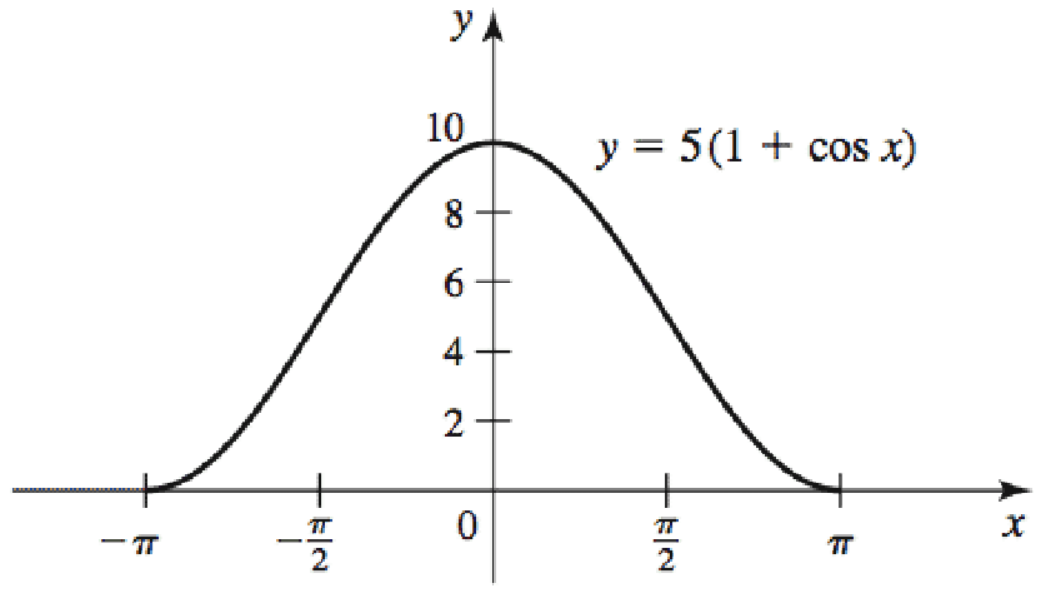
\includegraphics[scale=0.4]{exam4Sec5p4}

{\footnotesize Briggs, et. al. \emph{Calculus: Early Transcendentals, Second Edition.}}
\end{center}
\begin{solutionbox}
%\vspace
{2.85in}
Let $f(x)=5(1+\cos x)$.  The average value of $f$ on $[-\pi,\pi]$ is
\vspace{-0.5pc}
\begin{align*}
\bar f &= \frac{1}{\pi-(-\pi)}\int_{-\pi}^{\pi}5\underbrace{(1+\cos x)}_{\text{even function}}\ dx \\[0.1pc]
	&= \frac{1}{2\pi}\left(2\int_0^{\pi}5(1+\cos x)\ dx\right) \\[0.2pc]
	&= \left.\frac{5}{\pi}\left(x+\sin x\right)\right|_0^{\pi} \\[0.1pc]
	&= \frac{5}{\pi}\left(\pi+\sin{\pi}-(0+\sin 0)\right) \\[0.3pc]
	&= \frac{5}{\pi}(\pi+0-0-0)=\boxed{5}
\end{align*}
\end{solutionbox}
\vstr

% % % % % 
%\question[3] If $0<c<d$, then find the value of $b$ (in terms of $c$ and $d$) for which $\int_c^d(x+b)\ dx=0$.
%\vspace{3in}

% % % % %
%\question[1] Use geometry (not Riemann sums) to find the area and the net area of the region between the graph of $y=3x-6$ and the $x$-axis, for $0\leq x\leq 6$.
%\vspace{3in}
%\vstr

% % % % %
%\question[5.2]
%\begin{parts}
%\part[]\label{part:eval} Evaluate the definite integral $\int_0^{\frac{\pi}{2}}(2\sin{\theta}-\cos{\theta})\ d\theta$.
%\vspace{0.5in}

% % %
%\part[] Use your answer to part~\ref{part:eval} to evaluate $\int_{\frac{\pi}{2}}^0(4\cos{\theta}-8\sin{\theta})\ d\theta$.
%\vspace{0.5in}
%\end{parts}

% % % % % 
%\question[2] Use geometry (not Riemann sums) to evaluate the definite integral
%\[
%\int_0^{10}g(x)\ dx=\begin{cases} 4x & 0\leq x\leq 2 \\
%	-8x+16 & 2<x\leq 3 \\
%	-8 & x>3
%	\end{cases}.
%\]
%\vspace{4in}
%\vstr 

% % % % %
%\question[1] If $f$ is continuous on $[a,b]$ and $\int_a^b|f(x)|\ dx=0$, what can you conclude about $f$?
%\vspace{1in}

\newpage
% % % % % 
\fullwidth{
The Fundamental Theorem of Calculus says:
\begin{mdframed}
\begin{thm*}[Fundamental Theorem of Calculus] Suppose $f$ is continuous on $[a,b]$.
\vspace{-0.5pc}
\begin{itemize}
\item[I.] The area function $A(x)=\int_a^xf(t)\ dt$, for $a\leq x\leq b$, is continuous on $[a,b]$ and differentiable on $(a,b)$, and 
\vspace{-0.75pc}
\[
A'(x)=\frac{d}{dx}\int_a^xf(t)\ dt=f(x).
\]
\item[II.] If $F$ is any antiderivative of $f$ on $[a,b]$, then
\vspace{-0.75pc}
\[
\int_a^bf(x)\ dx=F(b)-F(a).
\]
\end{itemize}
\end{thm*}
\end{mdframed}
}
\vspace{-1pc}

% % % % %
\question Let $g(x)=\int_0^{\sin x}(t^2+1)\ dt$.  Compute $g'(x)$ using

\begin{parts}
% % %
\part[5] Part I of the Fundamental Theorem of Calculus.
\begin{solutionbox}
%\vspace
{0.6in}
\vspace{-2pc}
\[
g'(x)=\frac{d}{dx}\int_a^{\sin x}(t^2+1)\ dt=\boxed{\left((\sin x)^2+1\right)\cos x}
\]
\end{solutionbox}
\vstr

% % %
\part[5] Part II of the Fundamental Theorem of Calculus.
\begin{solutionbox}
%\vspace
{2.5in}
\vspace{-2pc}
\begin{align*}
g'(x) &= \frac{d}{dx}\int_a^{\sin x}(t^2+1)\ dt \\[0.2pc]
	&= \frac{d}{dx}\left(\left.\left(\frac{t^3}{3}+t\right)\right|_0^{\sin x}\right) \\[0.5pc]
	&= \frac{d}{dx}\left(\frac{(\sin x)^3}{3}+\sin x-\left(\frac{0^3}{3}-0\right)\right) \\[0.2pc]
	&= \frac{3}{3}(\sin x)^2(\cos x)+\cos x \\[0.2pc]
	&=\boxed{\left((\sin x)^2+1\right)\cos x}
\end{align*}
\end{solutionbox}
\vstr
\end{parts}
\vstr 

% % % % %
%\question[2] Find the value of $c$ such that the region bounded by $y=c\sin x$ and the $x$-axis on the interval $[0,\pi]$ has area $1$.
%\vspace{2in}
%
%\vstr

% % % % % % % % % % 
\newpage
\fullwidth{
The following table contains relevant formulas for the next two questions:
\[
\begin{tabular}{ c | c }
\text{Riemann sums with $n$ rectangles for $f$ on $[a,b]$} & \text{$\Sigma$-shortcuts} \\
\hline
{$\!
\begin{aligned}
\text{LEFT: } & \sum_{k=1}^nf(a+(k-1)\Delta x)\Delta x \\
\text{RIGHT: } & \sum_{k=1}^nf(a+k\Delta x)\Delta x
\end{aligned}
$}
& 
{$\!
\begin{aligned}
\sum_{k=1}^nc &= cn\quad\text{($c$ is a constant)} \\
\sum_{k=1}^nk &= \frac{n(n+1)}{2} \\
\end{aligned}
$}\\
%
\end{tabular}
\]
}

% % % % %
\question[10] Evaluate the left and right Riemann sums for $f$ over the interval $[1,5]$ for $n=8$.  
\[
\begin{tabular}{ |c|c|c|c|c|c|c|c|c|c| } 
 \hline
 $\vect x$ & 1 & 1.5 & 2 & 2.5 & 3 & 3.5 & 4 & 4.5 & 5 \\ 
 \hline
 $\vect{f(x)}$ & 0 & 2 & 3 & 2 & 2 & 1 & 0 & 2 & 3 \\ 
 \hline
\end{tabular}
\]
You are not required to use $\Sigma$-notation on this problem. 
\begin{solutionbox}
%\vspace
{2.5in}
For both sums, $\Delta x=\frac{b-a}{n}=\frac{5-1}{8}=\left(\frac{1}{2}\right)$.
\vspace{-1pc}
\begin{align*}
\text{LEFT:}\quad & \left(f(1)+f(1.5)+f(2)+f(2.5)+f(3)+f(3.5)+f(4)+f(4.5)\right)\left(\frac{1}{2}\right) \\
	=& \left(0+2+3+2+2+1+0+2\right)\left(\frac{1}{2}\right)=\frac{12}{2}=\boxed{6} \\[0.2pc]
\text{RIGHT:}\quad & \text{ LEFT}-f(1)\left(\frac{1}{2}\right)+f(5)\left(\frac{1}{2}\right) \\[0.2pc]
		= & \ 6-\frac{0}{2}+\frac{3}{2} = \boxed{\frac{15}{2}}
\end{align*}
\end{solutionbox}
\vstr

\newpage
% % % % %
\bonusquestion {\bf EXTRA CREDIT!}  Evaluate the following sums using $\Sigma$-notation.
 
\begin{parts}
% % % 
\bonuspart[2] $1+3+5+7+\cdots +99$
\begin{solutionbox}
%\vspace
{1.5in}
\vspace{-1.75pc}
\begin{align*}
\sum_{k=1}^{50}(2k-1) &= 2\sum_{k=1}^{50}k-\sum_{k=1}^{50}1 \\[0.2pc]
	&= 2\left(\frac{50(50+1)}{2}\right)-1(50) \\[0.1pc]
	&= 50(50)+50-50 = \boxed{2500}
\end{align*}
\end{solutionbox}
\vstr

% % %
\bonuspart[3] $4+9+14+\cdots +44$
\begin{solutionbox}
%\vspace
{1.75in}
\vspace{-1.75pc}
\begin{align*}
\sum_{k=1}^9(5k-1) &= 5\sum_{k=1}^9k-\sum_{k=1}^91 \\[0.2pc]
	&= 5\left(\frac{9(10)}{2}\right)-1(9) \\[0.1pc]
	&= 25(9)-1(9) \\
	&= 24(9)=\boxed{216}
\end{align*}
\end{solutionbox}
\vstr
% % %
%\bonuspart $3+8+13+\cdots +63$
%\vspace{1in}

% % %
%\part[] $\frac{1}{1\cdot 2}+\frac{1}{2\cdot 3}+\frac{1}{3\cdot 4}+\cdots+\frac{1}{49\cdot 50}$
%\vspace{0.5in}
\end{parts}
%\vstr

\end{questions}

\end{document}